\documentclass[11pt,a4paper]{article}

\usepackage[UTF8,fontset=mac]{ctex}
\usepackage[margin=2.5cm]{geometry}
\usepackage{amsmath,amssymb}
\usepackage{booktabs}
\usepackage{longtable}
\usepackage{graphicx}
\usepackage{float}
\usepackage{caption}
\usepackage{array}
\usepackage{xcolor}
\usepackage[colorlinks=true,linkcolor=blue!45!black,urlcolor=blue!45!black]{hyperref}

\captionsetup{font=small,labelsep=quad}
\setlength{\parskip}{0.3em}
\setlength{\parindent}{2em}
\linespread{1.12}

\newcommand{\SP}{S\&P~500}
\newcommand{\MOM}{\mathit{MOM}}

\title{\bfseries \SP{} 成分股 63 日动量因子的 20 日预测有效性}
\author{QuantToolKit 研究笔记}
\date{2026 年 10 月 22 日}

\begin{document}

\maketitle

\begin{abstract}
\noindent
本文使用 QuantToolKit 数据库中的日行情, 检验 63 个交易日的动量因子能否预测当前 \SP{} 成员未来 20 个交易日的收益。
样本包含数据库当前的 503 只成分股, 有效截面从 2016-04-05 到 2026-09-10, 共计 2{,}624 个, 日均截面约 485 只股票。
本文分别对原始动量和按 GICS 子行业中性化的动量计算每日 Pearson IC 与 Spearman Rank IC。
由于 20 日标签逐日重叠, IC 序列的一阶自相关达到 0.919 至 0.939, 本文使用 Bartlett 核、最大滞后 20 期的 Newey-West 协方差做推断。
结果显示, 原始 Rank IC 均值为 $-0.0133$, 行业中性 Rank IC 均值为 $-0.0057$, Newey-West $z$ 值分别为 $-1.10$ 和 $-0.96$, 均不显著。
若忽略重叠标签, 朴素 $t$ 值会达到 $-3.67$ 和 $-3.26$, 错误地给出显著结论。
按 Bartlett 权重折算的有效独立样本约为 196 至 236 个, 而不是 2{,}624 个。
非重叠抽样、前后分段、分年度以及 Newey-West 滞后阶数敏感性检验都不改变上述结论。
分位组合的 $Q5-Q1$ 20 日平均价差为 $-19.4$ 个基点, Newey-West $z=-0.62$, 同样不显著。
覆盖方面, 503 只当前成员中有 502 只至少有一天可以计算因子, 501 只至少有一天能得到完整的因子与标签。
综合来看, 在当前数据库的当前成分股面板上, 63 日动量对 20 日未来收益没有可靠的正向预测能力。

\vspace{0.6em}
\noindent\textbf{关键词:} 动量因子; 截面 IC; ICIR; 重叠标签; Newey-West; \SP
\end{abstract}

\tableofcontents
\newpage

\section{研究问题与计算口径}

\subsection{研究问题}

本文检验一个具体的可证伪问题: 对当前数据库内的 \SP{} 成员, 过去约一个季度涨得更多的股票, 在接下来约一个月是否继续涨得更多。
这里不做组合回测, 只做因子有效性的统计检验, 即计算因子值与未来收益的截面相关, 并处理重叠标签带来的序列相关。
研究对象是数据库中的当前成分股快照, 不是历史 \SP{} 全样本。

\subsection{因子定义}

设 $P_{i,t}$ 为股票 $i$ 在交易日 $t$ 的复权收盘价, 单期对数收益为 $r_{i,t}=\ln(P_{i,t}/P_{i,t-1})$。
63 日动量定义为：

\begin{equation}
\MOM_{63,i,t}
= \ln\frac{P_{i,t}}{P_{i,t-63}}
= \sum_{k=0}^{62} r_{i,t-k}
\label{eq:mom}
\end{equation}

该因子在 $t$ 日收盘后可得, 只使用 $t-63$ 到 $t$ 的价格。
计算按每只股票自己的交易记录计数, 不补齐交易日。
入库时首尾之间的缺口已经用前收盘价补齐, 这些补齐日的单期对数收益为 0, 会进入式~\eqref{eq:mom} 的求和。

行业中性动量在每个交易日按 GICS 子行业减去同行业均值：

\begin{equation}
\MOM^{\mathrm{ind}}_{i,t}
= \MOM_{63,i,t}
- \frac{1}{|G_t(i)|}\sum_{j\in G_t(i)}\MOM_{63,j,t}
\label{eq:neutral}
\end{equation}

其中 $G_t(i)$ 是 $t$ 日与股票 $i$ 属于同一 GICS 子行业且有有效因子值的股票集合。
行业中性化去掉了同行业共同的收益成分, 使不同行业的动量可以直接比较。
若某个子行业当天只有一只股票, 中性化后的值恒为 0, 这一点在解释中性 IC 时需要留意。

\subsection{标签与时间对齐}

标签是未来 20 个交易日的简单收益：

\begin{equation}
R_{i,t}^{(20)}
= \frac{P_{i,t+21}}{P_{i,t+1}}-1
\label{eq:label}
\end{equation}

即 $t$ 日收盘后得到因子, $t+1$ 日收盘入场, $t+21$ 日收盘出场, 对应代码中的 n\_periods = 20, gap = 1。
这样标签使用的 20 个日收益 $r_{i,t+2},\dots,r_{i,t+21}$ 与因子窗口 $r_{i,t-62},\dots,r_{i,t}$ 不重叠, 不存在同一日收益同时进入因子和标签的问题。
因子在 $t$ 日有效需要 64 条价格记录, 标签在 $t$ 日有效还需要之后 21 条记录, 因此一只股票从第 85 条价格记录起才会产生第一对完整的因子与标签。

\subsection{数据}

数据来自项目 DuckDB 数据库 data/quanttoolkit.db 中的 universe 与 prices 表。
universe 保存最近一次抓取的 \SP{} 成员名单, prices 保存日行情。
表~\ref{tab:coverage} 汇总了样本覆盖。
所有计算只读取数据库, 不写回。

\begin{table}[H]
\centering
\caption{数据与有效样本覆盖}
\label{tab:coverage}
\begin{tabular}{lr}
\toprule
项目 & 数值 \\
\midrule
当前 \SP{} 成员数 & 503 \\
有行情记录的股票数 & 503 \\
GICS 子行业数 & 126 \\
行情日期范围 & 2016-01-04 至 2026-10-09 \\
交易日数 & 2{,}708 \\
行情记录数 & 1{,}315{,}667 \\
复权收盘价缺失数 & 0 \\
成交量为 0 的补齐日记录数 & 2{,}743 \\
\addlinespace
至少一天可计算 $\MOM_{63}$ 的股票数 & 502 \\
至少一天有完整因子与标签的股票数 & 501 \\
完全无法进入有效样本的股票数 & 2 \\
\addlinespace
有效因子的首个交易日 & 2016-04-05 \\
有效标签的最后一个交易日 & 2026-09-10 \\
有效截面数 & 2{,}624 \\
有效样本的股票--日记录数 & 1{,}273{,}494 \\
每日截面股票数均值 & 485.3 \\
每日截面股票数范围 & 464 至 501 \\
\bottomrule
\end{tabular}
\end{table}

需要强调, universe 是当前成员名单, 不是历史成分股名单。
所有 2016 年以来的行情都是为当前成员回溯下载的, 期间被剔除或退市的公司不在样本内。
因此本文结果的对象是“当前 503 只成员构成的面板”, 不能直接外推为历史 \SP{} 的无条件结论。
这一幸存者偏差的方向并不显然: 它既可能保留长期赢家, 也可能漏掉曾经高动量、随后暴跌并被剔除的股票。

\section{样本覆盖: 哪些股票能被识别}

\subsection{“可识别”的两种含义}

“一只股票能否被动量因子识别”可以有两种含义。
第一种是数据覆盖意义上的可计算: 该股票在某个交易日同时有有效的 $\MOM_{63}$ 和已经实现的 20 日标签, 因而可以进入截面 IC 的计算。
第二种是预测意义上的可区分: 因子值能够稳定地区分它未来的高收益与低收益状态。
本节回答第一种含义, 第四节的统计结果回答第二种含义。
两者不能混同: 一只股票可以被稳定地计算因子, 但因子对它未来收益没有预测力。

\subsection{覆盖统计}

表~\ref{tab:coverage} 给出了总体覆盖。
503 只当前成员全部有行情记录, 复权收盘价没有缺失。
其中 502 只至少有一天可以计算 63 日动量, 501 只至少有一天能同时得到因子和 20 日标签。
没有任何完整样本的只有两只: HONA 和 VYLR。
HONA 从 2026-06-15 开始有行情, 2026-09-15 起才凑够 64 条记录可以计算因子, 但数据库最后一天是 2026-10-09, 之后 21 条记录无法取得, 所以没有实现的标签。
VYLR 从 2026-10-01 才开始有行情, 一共只有 7 条记录, 连 63 日动量都无法计算。
另有 FDXF 从 2026-05-27 开始交易, 只贡献了 11 个有效样本。

从时间维度看, 有完整历史的 464 只股票从 2016-04-05 起就进入截面, 其余 39 只晚上市股票在各自积累到第 85 条价格记录后陆续进入。
图~\ref{fig:coverage} 显示每日截面股票数从 464 只逐步增加到 501 只, 平均 485.3 只, 占当前成员总数的 96.5\%。
晚上市股票的完整清单、首个有效样本日和有效样本数见附录~\ref{app:late}。

\begin{figure}[H]
\centering
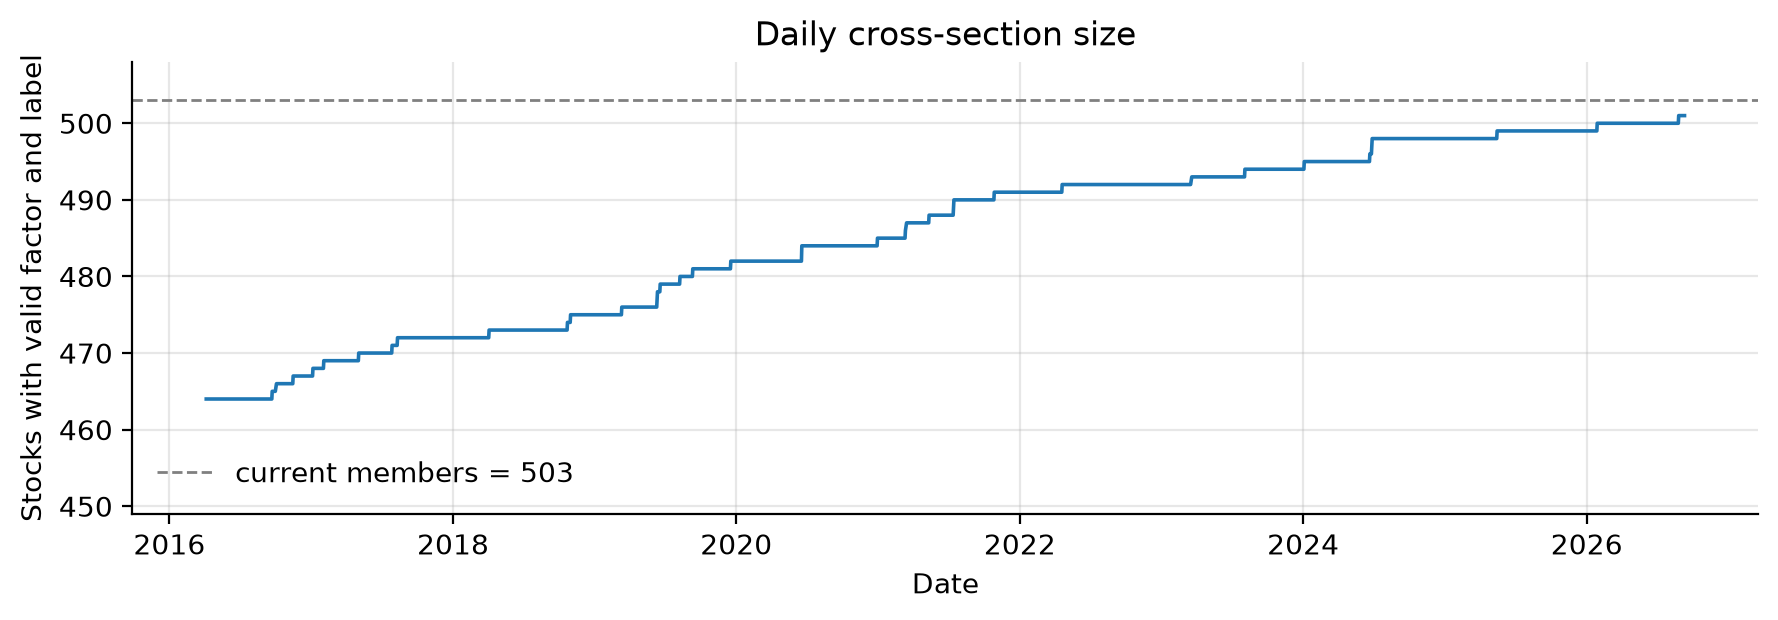
\includegraphics[width=0.92\textwidth]{figures/fig_coverage.png}
\caption{每日有有效因子和标签的股票数, 虚线是当前 503 只成员}
\label{fig:coverage}
\end{figure}

\section{研究方法}

\subsection{每日 IC 与 Rank IC}

对每个交易日 $t$, 在当天同时有有效因子值和有效标签的股票上计算截面相关：

\begin{align}
IC_t &= \operatorname{corr}_i\left(\MOM_{63,i,t},\,R_{i,t}^{(20)}\right), \label{eq:ic}\\
RankIC_t &= \operatorname{corr}_i\left(\operatorname{rank}(\MOM_{63,i,t}),\,\operatorname{rank}(R_{i,t}^{(20)})\right) \label{eq:rankic}
\end{align}

其中 $IC_t$ 是 Pearson 相关, $RankIC_t$ 是 Spearman 秩相关, 并列值取平均秩。
原始动量和行业中性动量分别计算这两个序列, 共四条 IC 序列。
样本中每个有效截面的股票数在 464 至 501 之间, 远大于计算相关所需的最小样本, 因此每天都能得到 IC 值, 没有缺失。

IC 序列的均值和样本标准差给出：

\begin{equation}
\overline{IC}=\frac{1}{T}\sum_{t=1}^{T}IC_t,\qquad
ICIR=\frac{\overline{IC}}{s(IC)}
\label{eq:icir}
\end{equation}

其中 $s(IC)$ 使用 ddof = 1。
ICIR 不做年化, 因为 20 日标签重叠, 把日频 ICIR 乘 $\sqrt{252}$ 没有意义。
本文同时报告 $IC>0$ 的比例, 它衡量方向稳定性。

\subsection{重叠标签与 Newey-West 推断}

$t$ 日与 $t+1$ 日的标签窗口分别是 $[t+1,t+21]$ 和 $[t+2,t+22]$, 共享 19 个日收益。
因此 IC 序列存在很强的序列相关, 用独立同分布假设下的朴素标准误：

\begin{equation}
\widehat{\mathrm{se}}_{\mathrm{naive}}=\frac{s(IC)}{\sqrt{T}}
\label{eq:naive}
\end{equation}

会严重低估均值的不确定性。
本文对均值方程 $IC_t=\mu+\varepsilon_t$ 使用 Newey-West 异方差自相关一致 (HAC) 协方差：

\begin{equation}
\widehat{\mathrm{Var}}_{\mathrm{HAC}}(\hat\mu)
=\frac{1}{T^2}\sum_{t=1}^{T}\sum_{s=1}^{T} w_{|t-s|}\,
(IC_t-\hat\mu)(IC_s-\hat\mu),
\qquad
w_k=\max\left(0,\,1-\frac{k}{L+1}\right)
\label{eq:nw}
\end{equation}

其中 $w_k$ 是 Bartlett 核权重, 最大滞后 $L=20$, 与 20 日标签的重叠长度一致。
检验统计量为 $z=\hat\mu/\widehat{\mathrm{se}}_{\mathrm{HAC}}$, 双侧 $p$ 值按标准正态分布计算, 与项目现有代码中 use\_t = False 的设定一致。
同时用 Bartlett 权重下的自相关和估计有效独立样本：

\begin{equation}
T_{\mathrm{eff}}
=\frac{T}{1+2\sum_{k=1}^{L}\left(1-\frac{k}{L+1}\right)\hat\rho_k}
\label{eq:teff}
\end{equation}

其中 $\hat\rho_k$ 是 IC 序列的 $k$ 阶自相关。
$T_{\mathrm{eff}}$ 用来直观说明重叠标签使“等价样本量”从 2{,}624 降到 200 左右。

\subsection{稳健性设计}

为确认结论不依赖某一种设定, 本文做四组检查：

\begin{enumerate}
\item 把 Newey-West 最大滞后分别取 5, 10, 20, 40, 60, 120, 观察 $z$ 值是否稳定。
\item 每 20 个交易日抽取一个截面, 近似构造非重叠样本, 此时普通 $t$ 统计量可以作为交叉验证。
\item 按时间等分前后两段, 分别用 Newey-West 推断, 观察方向和显著性的稳定性。
\item 按日历年汇总 IC 均值, 观察预测力是否只集中在个别年份。
\end{enumerate}

最后用分位组合衡量经济幅度: 每个交易日按动量从低到高分成五组, 计算各组未来 20 日等权平均收益, 并检验 $Q5-Q1$ 的价差。
价差序列仍然使用最大滞后 20 期的 Newey-West 标准误。
由于所有检验都是单因子、日频截面, 本文对四条 IC 序列分别做推断, 未做多重检验校正; 所有 $p$ 值都较大, 校正不会改变结论。

\section{实证结果}

\subsection{IC 描述统计}

表~\ref{tab:icsummary} 给出四条 IC 序列的均值、标准差、ICIR、$IC>0$ 比例和朴素 $t$ 值。
所有 IC 均值在经济上都很小: 原始 IC 为 $-0.0056$, 中性 IC 为 $0.0012$, 原始 Rank IC 为 $-0.0133$, 中性 Rank IC 为 $-0.0057$。
ICIR 在 $-0.0716$ 到 $0.0089$ 之间。
$IC>0$ 的比例在 49.5\% 到 54.2\% 之间, 接近抛硬币。
单看均值, 原始动量略偏负, 行业中性化后几乎回到 0, 没有出现动量因子应有的正 IC。

\begin{table}[H]
\centering
\caption{每日 IC 序列的描述统计}
\label{tab:icsummary}
\begin{tabular}{lrrrrrr}
\toprule
指标 & 交易日数 & 均值 & 标准差 & ICIR & $IC>0$ 比例 & 朴素 $t$ \\
\midrule
原始 IC & 2{,}624 & $-0.005623$ & 0.200567 & $-0.0280$ & 0.5366 & $-1.436$ \\
中性 IC & 2{,}624 & $0.001180$ & 0.132758 & $0.0089$ & 0.5419 & $0.455$ \\
原始 Rank IC & 2{,}624 & $-0.013300$ & 0.185854 & $-0.0716$ & 0.5076 & $-3.666$ \\
中性 Rank IC & 2{,}624 & $-0.005653$ & 0.088948 & $-0.0636$ & 0.4950 & $-3.256$ \\
\bottomrule
\end{tabular}
\end{table}

表中朴素 $t$ 值按式~\eqref{eq:naive} 计算, 它假设每日 IC 相互独立。
原始 Rank IC 和中性 Rank IC 的朴素 $t$ 值都低于 $-3$, 如果直接看这个数字, 会得到“动量显著为负”的结论。
这个结论是重叠标签造成的伪显著, 下一小节给出修正结果。

\subsection{Newey-West 修正后的推断}

表~\ref{tab:nw} 给出最大滞后 20 期的 Newey-West 标准误、$z$ 值、双侧 $p$ 值和 95\% 置信区间。
修正后的标准误是朴素标准误的 3.33 到 3.66 倍, 四个 $z$ 值的绝对值都不超过 1.10, $p$ 值在 0.272 到 0.901 之间。
四个 95\% 置信区间都包含 0, 而且区间宽度在经济上不可忽略。
例如原始 Rank IC 的 95\% 置信区间是 $[-0.0370,\,0.0104]$, 既不能排除温和的负向关系, 也不能排除温和的正向关系。

\begin{table}[H]
\centering
\caption{Newey-West 修正后的 IC 均值推断 (最大滞后 20 期)}
\label{tab:nw}
\begin{tabular}{lrrrrr}
\toprule
指标 & 均值 & NW 标准误 & $z$ 值 & $p$ 值 & 95\% 置信区间 \\
\midrule
原始 IC & $-0.005623$ & 0.013744 & $-0.409$ & 0.682 & $[-0.0326,\,0.0213]$ \\
中性 IC & $0.001180$ & 0.009482 & $0.124$ & 0.901 & $[-0.0174,\,0.0198]$ \\
原始 Rank IC & $-0.013300$ & 0.012099 & $-1.099$ & 0.272 & $[-0.0370,\,0.0104]$ \\
中性 Rank IC & $-0.005653$ & 0.005920 & $-0.955$ & 0.340 & $[-0.0173,\,0.0059]$ \\
\bottomrule
\end{tabular}
\end{table}

修正前后差异的来源是 IC 序列的强自相关。
表~\ref{tab:acf} 给出 1, 5, 10, 15, 20 阶自相关和有效样本量。
四条序列的一阶自相关在 0.919 到 0.939 之间, 到第 15 阶仍有 0.071 到 0.256, 到第 20 阶附近才衰减到 0 附近。
按式~\eqref{eq:teff} 折算, 有效独立样本只有 195.9 到 235.8 个, 约为名义样本 2{,}624 的 7.5\% 到 9.0\%。
图~\ref{fig:acf} 直观展示了这种缓慢衰减。
这也是为什么对重叠标签直接套用普通 $t$ 检验会严重高估显著性。

\begin{table}[H]
\centering
\caption{IC 序列的自相关与有效样本量}
\label{tab:acf}
\begin{tabular}{lrrrrrr}
\toprule
指标 & $\hat\rho_1$ & $\hat\rho_5$ & $\hat\rho_{10}$ & $\hat\rho_{15}$ & $\hat\rho_{20}$ & $T_{\mathrm{eff}}$ \\
\midrule
原始 IC & 0.928 & 0.671 & 0.427 & 0.174 & $-0.061$ & 212.8 \\
中性 IC & 0.939 & 0.718 & 0.500 & 0.256 & $0.016$ & 195.9 \\
原始 Rank IC & 0.919 & 0.623 & 0.342 & 0.071 & $-0.154$ & 235.8 \\
中性 Rank IC & 0.924 & 0.641 & 0.380 & 0.112 & $-0.127$ & 225.6 \\
\bottomrule
\end{tabular}
\end{table}

\begin{figure}[H]
\centering
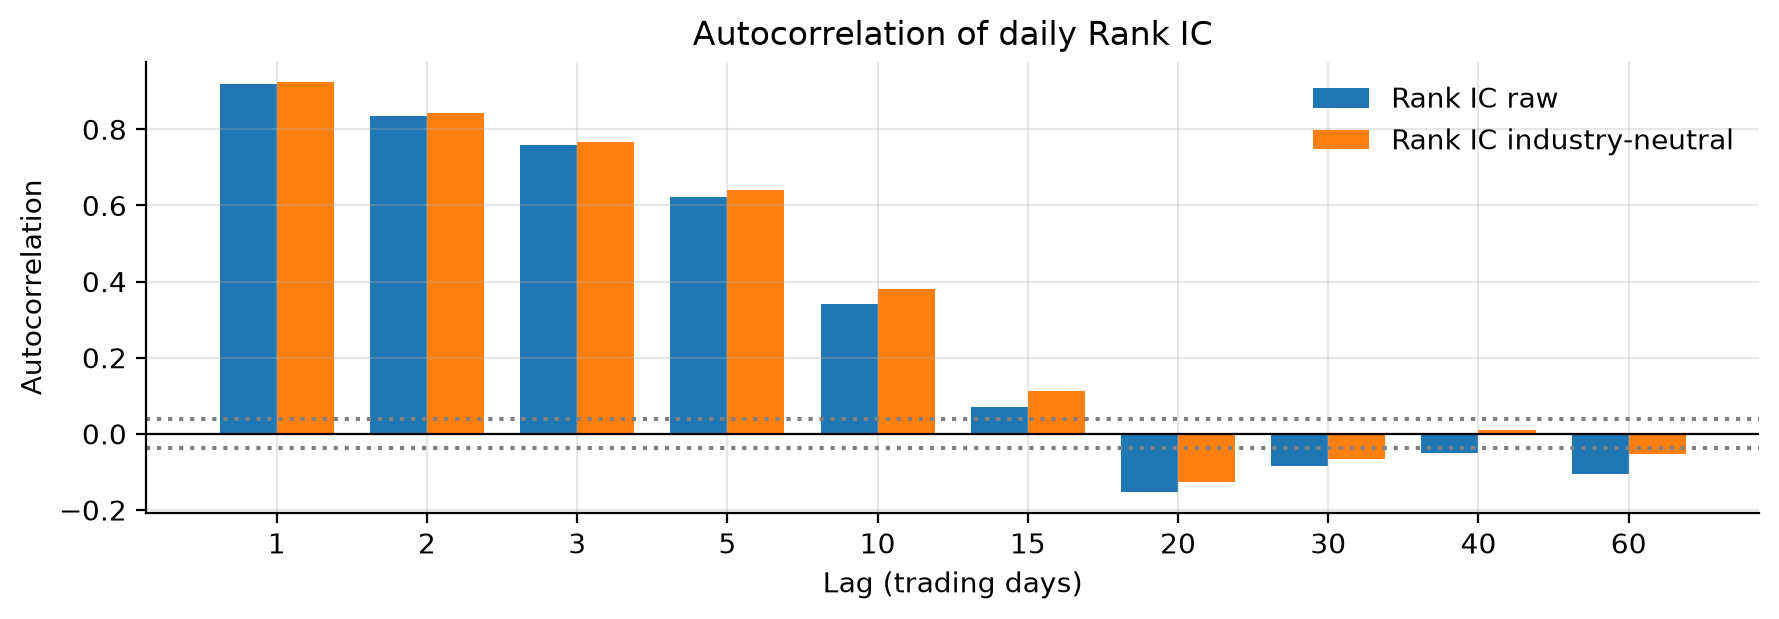
\includegraphics[width=0.92\textwidth]{figures/fig_acf.png}
\caption{每日 Rank IC 的自相关, 虚线是 $\pm1.96/\sqrt{T}$ 的独立同分布参考带}
\label{fig:acf}
\end{figure}

\subsection{稳健性检验}

\textbf{滞后阶数}：
表~\ref{tab:lag} 把 Newey-West 最大滞后从 5 改到 120。
原始 Rank IC 的 $z$ 值在 $-1.63$ 到 $-1.08$ 之间, 中性 Rank IC 的 $z$ 值在 $-1.44$ 到 $-0.91$ 之间, 都远未达到常用显著性水平。
从 20 期继续增加滞后, 结论基本不变, 说明 20 期已经捕捉了主要的重叠结构。

\begin{table}[H]
\centering
\caption{Newey-West 最大滞后敏感性 ($z$ 值)}
\label{tab:lag}
\begin{tabular}{rrrrr}
\toprule
最大滞后 & 原始 IC & 中性 IC & 原始 Rank IC & 中性 Rank IC \\
\midrule
5   & $-0.631$ & $0.198$ & $-1.629$ & $-1.441$ \\
10  & $-0.496$ & $0.154$ & $-1.295$ & $-1.139$ \\
20  & $-0.409$ & $0.124$ & $-1.099$ & $-0.955$ \\
40  & $-0.384$ & $0.114$ & $-1.076$ & $-0.917$ \\
60  & $-0.384$ & $0.111$ & $-1.108$ & $-0.910$ \\
120 & $-0.435$ & $0.112$ & $-1.357$ & $-1.007$ \\
\bottomrule
\end{tabular}
\end{table}

\textbf{非重叠抽样与分段样本}：
表~\ref{tab:robust} 汇总了四种样本设定下的 Rank IC。
每 20 个交易日抽样后得到 132 个近似非重叠截面, 原始 Rank IC 均值为 $-0.0098$ ($t=-0.66$), 中性为 $-0.0056$ ($t=-0.76$), 都不显著。
按时间等分后, 前半段 (2016-04-05 至 2021-06-18) 原始 Rank IC 为 $-0.0101$ ($z=-0.59$), 中性为 $-0.0115$ ($z=-1.49$)。
后半段 (2021-06-21 至 2026-09-10) 原始 Rank IC 为 $-0.0165$ ($z=-0.98$), 中性为 $0.0002$ ($z=0.03$)。
原始动量的符号在前后两段都偏负但不显著, 中性动量的符号则发生了翻转, 没有稳定方向。

\begin{table}[H]
\centering
\caption{Rank IC 在不同样本设定下的稳健性}
\label{tab:robust}
\small
\begin{tabular}{lrrrrr}
\toprule
样本 & 截面数 & 原始 Rank IC & $z$ 或 $t$ & 中性 Rank IC & $z$ 或 $t$ \\
\midrule
全样本 (NW, $L=20$) & 2{,}624 & $-0.0133$ & $-1.099$ & $-0.0057$ & $-0.955$ \\
每 20 个交易日抽样 & 132 & $-0.0098$ & $-0.657$ & $-0.0056$ & $-0.762$ \\
前半段 2016-04 至 2021-06 & 1{,}312 & $-0.0101$ & $-0.585$ & $-0.0115$ & $-1.491$ \\
后半段 2021-06 至 2026-09 & 1{,}312 & $-0.0165$ & $-0.977$ & $0.0002$ & $0.026$ \\
\bottomrule
\end{tabular}
\end{table}

\textbf{分年度结果}：
表~\ref{tab:yearly} 和图~\ref{fig:ic} 给出分年度均值。
原始 Rank IC 在 2017, 2020, 2024 年为正, 其余年份为负, 符号在年份之间来回切换。
最强的正向年份是 2024 年 ($0.0232$), 最强的负向年份是 2023 年 ($-0.0514$) 和 2026 年部分年度 ($-0.0450$)。
中性 Rank IC 的波动更小, 也没有连续的正向年份。
把 60 日滚动均值画出来后, 可以看到 IC 在 0 附近做长周期摆动, 没有持续的正向区间。
这是典型的“某几年看起来能用, 换一段样本就失效”的形态。

\begin{table}[H]
\centering
\caption{分年度 IC 均值}
\label{tab:yearly}
\begin{tabular}{rrrrrr}
\toprule
年份 & 截面数 & 原始 IC & 中性 IC & 原始 Rank IC & 中性 Rank IC \\
\midrule
2016 & 189 & $-0.0257$ & $-0.0302$ & $-0.0352$ & $-0.0290$ \\
2017 & 251 & $0.0195$ & $0.0113$ & $0.0231$ & $0.0057$ \\
2018 & 251 & $0.0109$ & $0.0299$ & $-0.0102$ & $0.0006$ \\
2019 & 252 & $-0.0673$ & $-0.0687$ & $-0.0313$ & $-0.0238$ \\
2020 & 253 & $0.0008$ & $-0.0080$ & $0.0115$ & $-0.0087$ \\
2021 & 252 & $-0.0345$ & $0.0065$ & $-0.0349$ & $0.0081$ \\
2022 & 251 & $0.0055$ & $0.0164$ & $-0.0056$ & $-0.0020$ \\
2023 & 250 & $-0.0443$ & $-0.0366$ & $-0.0514$ & $-0.0229$ \\
2024 & 252 & $0.0350$ & $0.0431$ & $0.0232$ & $0.0177$ \\
2025 & 250 & $0.0336$ & $0.0323$ & $-0.0061$ & $-0.0048$ \\
2026 & 173 & $0.0022$ & $0.0132$ & $-0.0450$ & $-0.0105$ \\
\bottomrule
\end{tabular}
\end{table}

\begin{figure}[H]
\centering
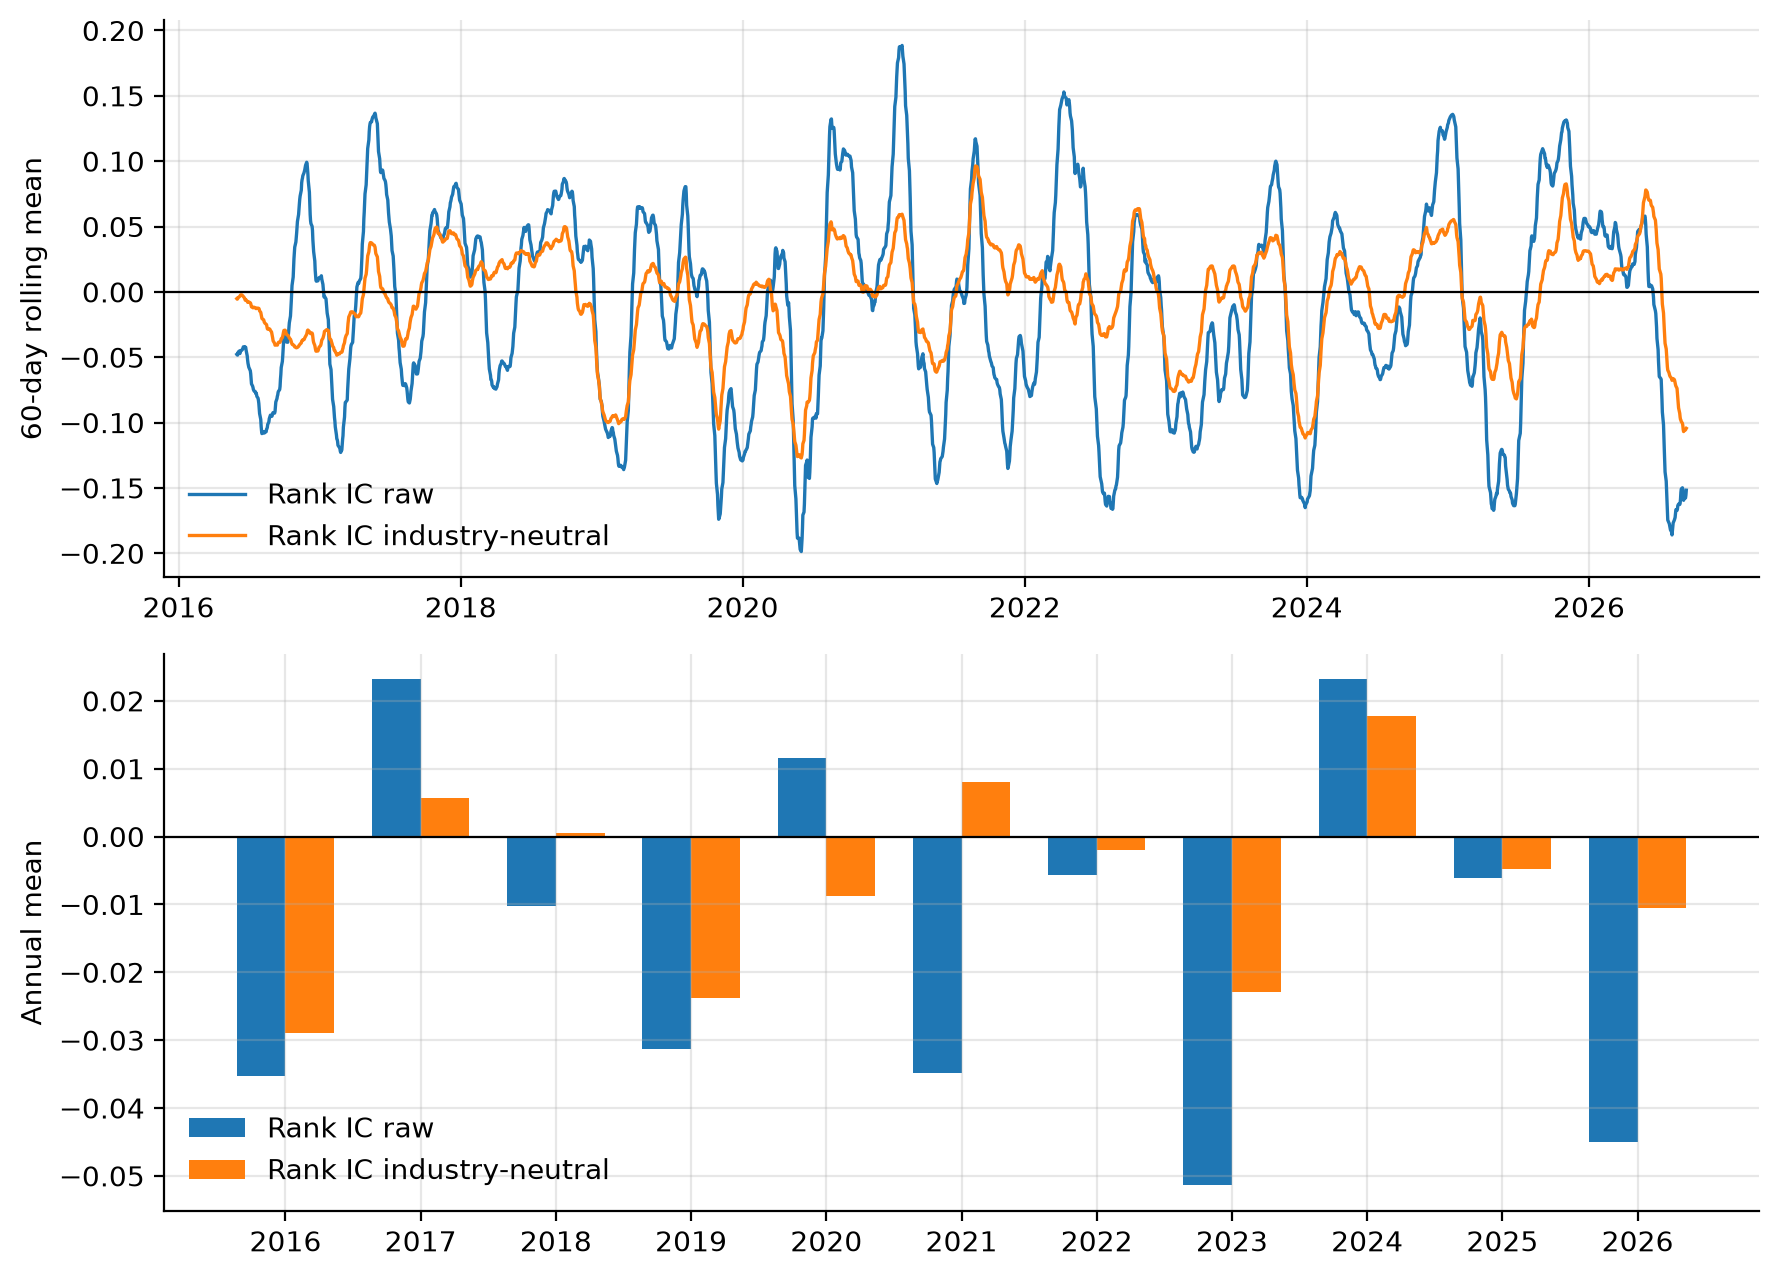
\includegraphics[width=0.9\textwidth]{figures/fig_ic.png}
\caption{上: Rank IC 的 60 日滚动均值; 下: 分年度 Rank IC 均值}
\label{fig:ic}
\end{figure}

\subsection{分位组合}

表~\ref{tab:quintile} 给出按动量分五组后各组未来 20 日的等权平均收益。
若动量有效, 收益应随分组单调上升, $Q5$ 最高, $Q1$ 最低。
实际结果是 $Q1$ (最低动量) 反而最高, 原始动量为 1.740\%, 中性动量为 1.688\%, $Q5$ 分别为 1.547\% 和 1.601\%, 中间三组在 1.22\% 到 1.34\% 之间。
整体没有单调关系。

\begin{table}[H]
\centering
\caption{按动量分组的未来 20 日等权平均收益 (\%)}
\label{tab:quintile}
\begin{tabular}{lrr}
\toprule
分组 & 原始动量 & 行业中性动量 \\
\midrule
$Q1$ (最低) & 1.740 & 1.688 \\
$Q2$ & 1.337 & 1.285 \\
$Q3$ & 1.234 & 1.290 \\
$Q4$ & 1.225 & 1.217 \\
$Q5$ (最高) & 1.547 & 1.601 \\
\bottomrule
\end{tabular}
\end{table}

表~\ref{tab:spread} 给出 $Q5-Q1$ 价差的 Newey-West 推断。
原始动量的 20 日价差为 $-19.35$ 个基点 ($z=-0.616$, $p=0.538$), 中性动量为 $-8.72$ 个基点 ($z=-0.496$, $p=0.620$)。
价差的方向与动量相反, 但幅度不显著, 不能据此认为存在稳定的反转, 只能说不存在动量溢价。
图~\ref{fig:quintile} 展示了同一结果。

\begin{table}[H]
\centering
\caption{$Q5-Q1$ 未来 20 日平均价差的 Newey-West 推断}
\label{tab:spread}
\begin{tabular}{lrrrrr}
\toprule
因子 & 均值 (bps) & NW 标准误 (bps) & $z$ 值 & $p$ 值 & 95\% 置信区间 (bps) \\
\midrule
原始动量 & $-19.35$ & 31.42 & $-0.616$ & 0.538 & $[-80.94,\,42.23]$ \\
行业中性动量 & $-8.72$ & 17.58 & $-0.496$ & 0.620 & $[-43.17,\,25.73]$ \\
\bottomrule
\end{tabular}
\end{table}

\begin{figure}[H]
\centering
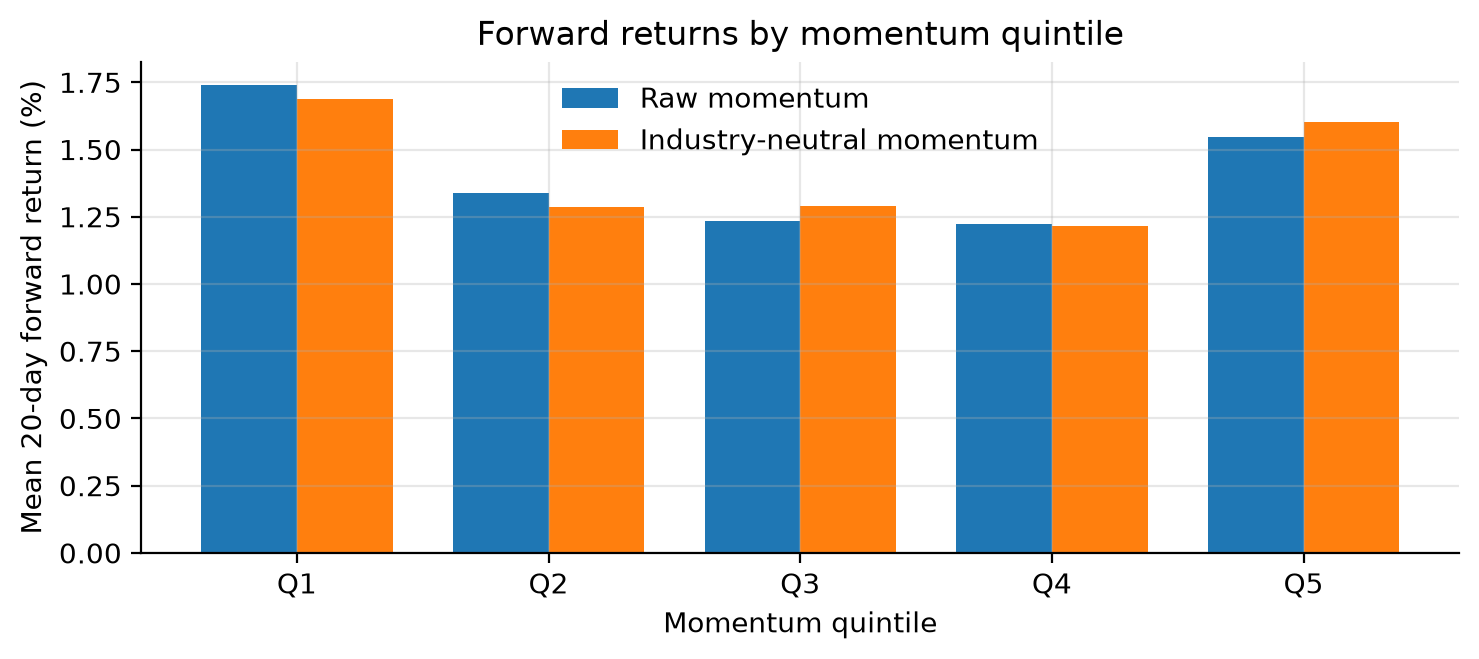
\includegraphics[width=0.75\textwidth]{figures/fig_quintile.png}
\caption{按动量五分组的未来 20 日等权平均收益}
\label{fig:quintile}
\end{figure}

\section{讨论}

\subsection{为什么没有观察到动量}

本文的结果与“大盘股、短持有期上动量较弱”的经验一致, 但具体原因需要更细的分解才能确定。
下面列出几种合理解释, 以及它们与本文设定的关系：

\begin{enumerate}
\item \textbf{持有期偏短}：
20 个交易日约一个月, 而经典动量溢价通常用 3 到 12 个月的形成期和持有期衡量。
在一个月的尺度上, 短期反转的力量可能盖过动量。

\item \textbf{形成期包含最近一个月}：
本文按目标文档使用 63 日形成期且 skip = 0, 因子包含最近 21 个交易日的收益。
经典 12-1 动量会跳过最近一个月, 以避免短期反转污染。
因此本文的因子更接近“季度动量加短期反转”的混合, 这可能是正向预测力缺失的原因之一。
本文没有正式检验 skip 变体, 这一点留作后续工作。

\item \textbf{行业中性化去掉了行业轮动}：
行业中性化按子行业减去均值, 会移除行业层面的共同动量。
不过原始动量的结果同样不显著, 所以行业中性化不是唯一原因。

\item \textbf{样本期包含多次风格切换}：
2016 至 2026 年包含 2020 年疫情冲击、2022 年成长股回撤和 2023 年之后的大盘科技股行情。
这些阶段的动量表现差异很大, 分年度结果也显示符号频繁翻转。

\item \textbf{幸存者偏差}：
股票池是当前成员, 被剔除或退市的公司不在样本内。
这会改变横截面的收益分布, 对动量结论的影响方向不确定。
因此本文结论只适用于当前成员面板。

\item \textbf{单因子与无成本设定}：
本文只计算单因子截面 IC 和等权分位收益, 没有控制市值、流动性、波动率和估值, 也没有扣除交易成本。
IC 不显著意味着即使做多空组合也很难覆盖成本, 但本文没有做完整的组合回测。
\end{enumerate}

\subsection{如何理解“哪些股票能被识别”}

从数据覆盖看, 答案是清楚的: 当前 503 只成员中, 502 只至少有一天可以计算 63 日动量, 501 只至少有一天可以同时得到因子和标签。
每日可用的截面从 464 只增加到 501 只, 平均 485.3 只。
附录~\ref{app:late} 列出了 39 只晚上市股票及其首个有效样本日。

从预测意义看, 答案是否定的: 本文没有发现动量因子能够稳定地区分未来 20 日的高收益和低收益股票。
如果强行按某一天的动量排名挑出“高动量股票”, 这些股票在样本内并没有系统性地跑赢低动量股票。
因此不能把“因子可计算”误读为“因子有识别力”。

\subsection{局限}

\begin{itemize}
\item 股票池是当前成员快照, 存在幸存者偏差, 不能外推到历史 \SP。
\item 有效样本期只有 2016-04 至 2026-09, 共 2{,}624 个截面, 约 10.7 年, 不足以覆盖完整的长周期。
\item 行情来自 Yahoo 复权收盘价, 补齐日的零收益会轻微平滑动量。
\item 子行业中性化在单股票子行业上恒为 0, 会稀释中性因子的截面差异。
\item 只检验 20 日持有期, 没有检验 1 个月以上的持有期、换手率和交易成本。
\item 只做单因子分析, 没有控制市值、流动性、波动率等常见风险暴露。
\end{itemize}

\section{结论}

\begin{enumerate}
\item \textbf{覆盖}：
数据库当前 503 只 \SP{} 成员全部有行情, 其中 502 只至少有一天可计算 $\MOM_{63}$, 501 只至少有一天有完整的因子与标签。
每日截面平均 485.3 只, 从 2016 年的 464 只逐步增加到 2026 年的 501 只。

\item \textbf{预测力}：
原始 Rank IC 均值为 $-0.0133$, 行业中性 Rank IC 均值为 $-0.0057$, 数值很小且方向不稳定。
按最大滞后 20 期做 Newey-West 修正后, $z$ 值分别为 $-1.10$ 和 $-0.96$, $p$ 值为 0.272 和 0.340, 均不显著。

\item \textbf{重叠标签的重要性}：
日度 IC 的一阶自相关约 0.92, 有效独立样本只有约 196 至 236 个。
若不修正, 原始 Rank IC 的朴素 $t$ 值会达到 $-3.67$, 产生“显著为负”的伪结论。
处理重叠标签是这类 20 日因子检验中不可省略的一步。

\item \textbf{稳健性}：
非重叠抽样、前后分段、分年度和 Newey-West 滞后阶数敏感性检验都不支持稳定动量。
中性动量的符号在前后半段发生翻转, 分年度符号也频繁变化。

\item \textbf{经济幅度}：
$Q5-Q1$ 的 20 日平均价差为 $-19.4$ 个基点, Newey-West $z=-0.62$, 不显著。
低动量组反而略高, 但不足以确认稳定的反转效应。

\item \textbf{实践含义}：
在当前数据库的当前成分股样本上, 63 日动量不适合作为单独的多头选股信号。
它可以作为多因子模型的一个候选特征, 但需要更长样本、历史成分股、不同形成期和持有期, 以及样本外检验来确认。
\end{enumerate}

\appendix

\section{晚上市股票清单}
\label{app:late}

表~\ref{tab:late} 列出 2016-01-04 之后才有行情的 39 只当前成员。
“首个有效样本日”指第一对完整因子与 20 日标签的日期, 即第 85 条价格记录对应的交易日。
HONA 和 VYLR 在数据库最后一天之前没有凑齐完整样本, 因此标为无。

{\footnotesize
\renewcommand{\arraystretch}{0.95}
\begin{longtable}{@{}>{\raggedright\arraybackslash}p{1.1cm}>{\raggedright\arraybackslash}p{3.2cm}>{\raggedright\arraybackslash}p{5.4cm}>{\raggedright\arraybackslash}p{2.3cm}r@{}}
\caption{晚上市股票及其首个有效样本日}
\label{tab:late}\\
\toprule
代码 & 公司 & GICS 子行业 & 首个有效样本日 & 有效样本数 \\
\midrule
\endfirsthead
\toprule
代码 & 公司 & GICS 子行业 & 首个有效样本日 & 有效样本数 \\
\midrule
\endhead
\bottomrule
\endfoot
TWLO & Twilio & Systems Software & 2016-09-22 & 2505 \\
FTV & Fortive & Industrial Machinery \& Supplies \& Components & 2016-10-03 & 2498 \\
DELL & Dell Technologies & Technology Hardware, Storage \& Peripherals & 2016-11-15 & 2467 \\
VST & Vistra Corp. & Electric Utilities & 2017-01-05 & 2433 \\
HWM & Howmet Aerospace & Aerospace \& Defense & 2017-02-02 & 2414 \\
INVH & Invitation Homes & Single-Family Residential REITs & 2017-05-03 & 2352 \\
CVNA & Carvana & Automotive Retail & 2017-07-28 & 2292 \\
IR & Ingersoll Rand & Industrial Machinery \& Supplies \& Components & 2017-08-11 & 2282 \\
VICI & Vici Properties & Hotel \& Resort REITs & 2018-04-04 & 2121 \\
BE & Bloom Energy & Electrical Components \& Equipment & 2018-10-23 & 1980 \\
VRT & Vertiv & Electrical Components \& Equipment & 2018-10-31 & 1974 \\
MRNA & Moderna & Biotechnology & 2019-03-12 & 1886 \\
FOXA & Fox Corporation (Class A) & Broadcasting & 2019-06-11 & 1823 \\
FOX & Fox Corporation (Class B) & Broadcasting & 2019-06-12 & 1822 \\
DOW & Dow Inc. & Commodity Chemicals & 2019-06-19 & 1817 \\
UBER & Uber & Passenger Ground Transportation & 2019-08-09 & 1781 \\
CRWD & CrowdStrike & Systems Software & 2019-09-11 & 1759 \\
DDOG & Datadog & Application Software & 2019-12-18 & 1690 \\
CARR & Carrier Global & Building Products & 2020-06-18 & 1565 \\
OTIS & Otis Worldwide & Industrial Machinery \& Supplies \& Components & 2020-06-18 & 1565 \\
PLTR & Palantir Technologies & Application Software & 2020-12-30 & 1430 \\
DASH & DoorDash & Specialized Consumer Services & 2021-03-12 & 1381 \\
ABNB & Airbnb & Hotels, Resorts \& Cruise Lines & 2021-03-15 & 1380 \\
EXE & Expand Energy & Oil \& Gas Exploration \& Production & 2021-05-12 & 1339 \\
COIN & Coinbase & Financial Exchanges \& Data & 2021-07-14 & 1296 \\
APP & AppLovin & Advertising & 2021-07-15 & 1295 \\
HOOD & Robinhood Markets & Investment Banking \& Brokerage & 2021-10-27 & 1222 \\
CEG & Constellation Energy & Electric Utilities & 2022-04-20 & 1102 \\
GEHC & GE HealthCare & Health Care Equipment & 2023-03-20 & 873 \\
KVUE & Kenvue & Personal Care Products & 2023-08-04 & 778 \\
VLTO & Veralto & Environmental \& Facilities Services & 2024-01-04 & 673 \\
RDDT & Reddit & Interactive Media \& Services & 2024-06-21 & 557 \\
SOLV & Solventum & Health Care Technology & 2024-06-26 & 554 \\
GEV & GE Vernova & Heavy Electrical Equipment & 2024-06-27 & 553 \\
SNDK & Sandisk & Technology Hardware, Storage \& Peripherals & 2025-05-15 & 332 \\
Q & Qnity Electronics & Semiconductor Materials \& Equipment & 2026-01-28 & 156 \\
FDXF & FedEx Freight & Cargo Ground Transportation & 2026-08-26 & 11 \\
HONA & Honeywell Aerospace & Aerospace \& Defense & 无 & 0 \\
VYLR & Vylor & Agricultural Products \& Services & 无 & 0 \\
\end{longtable}
}

HONA 从 2026-09-15 起已经可以计算因子, 但数据库最后一天 2026-10-09 之前无法取得 20 日之后的价格, 所以没有实现的标签。
VYLR 只有 7 条价格记录, 无法计算 63 日动量。
其余 37 只晚上市股票在表~\ref{tab:late} 给出的日期之后都进入样本。

\section{复现说明}
\label{app:reproduce}

分析代码和全部中间结果都在 research/test\_momfactors 目录下：

\begin{itemize}
\item 分析 notebook: main.ipynb, 顺序执行即可重新生成全部表格和图片。
\item 报告: momfactor.tex, 使用 XeLaTeX 编译。
\item 图片: figures 目录下的 fig\_coverage.png, fig\_acf.png, fig\_ic.png, fig\_quintile.png。
\item 表格: outputs 目录下的 CSV 文件, 与正文表格一一对应。
\end{itemize}

运行环境为 Python 3.12.13, pandas 3.0.6, numpy 2.5.4, statsmodels 0.15.0, duckdb 1.5.6。
绘图与 notebook 执行使用 matplotlib 3.11.2 和 nbconvert 7.17.2, 这两个包是本次分析额外安装的, 未写入 pyproject.toml。
数据库路径由 quanttoolkit.db.connection.DB 给出, 默认为仓库根目录下的 data/quanttoolkit.db。
复现命令如下：

\begin{verbatim}
cd research/test_momfactors
jupyter nbconvert --to notebook --execute --inplace main.ipynb
xelatex momfactor.tex
xelatex momfactor.tex
\end{verbatim}

notebook 只读取数据库, 不修改任何行情或成员名单。
所有随机性均不涉及, 结果完全可复现。

\end{document}
